\subsection{Responsive Cyber Defence Requirements}
\label{sec:rcd}
\glsresetall
% RCD definition
\gls{rcd} is a controversial, vaguely understood and seldom used term. More commonly, a broader concept of \gls{acd} is utilized as presented in chapter \ref{sec:rcd-work}.
One definition states that \gls{acd} is accomplished through denial to information and deception via misleading information \cite{Heckman2013} \cite{Heckman2015}.
Another definition suggests actively engaging the incoming cyber attack to destroy or reduce its effectiveness \cite{Denning2014}, or conduct the hack-back \cite{Mansfield2009}.
Contrary to this, US DARPA acknowledges \gls{acd} (see footnote \ref{fnote:darpa} on page \pageref{fnote:darpa}) without the component of actively pursuing and interacting with the adversary.
Yet another \gls{acd} concept is directed to threat assessment and mitigation \cite{Dewar2017}.
Some view this approach purely limited to one set of approaches (e.g. \textit{``white worms''}, address hopping) \cite{Lu2013} \cite{Repik2008}.
One proposed \gls{rcd} definition is aimed at gaining access to the third-party systems for modification or deletion of data held therein \cite{Maybaum2014}.
Another \gls{rcd} definition is quite broad and permits any applicable defensive actions to be taken against any communication and information system engaged or used in the attack \cite{Brangetto2014-2}.
These various definitions of \gls{acd} are mainly focused towards the integrated and synchronized real-time capability for detection, analysis, identification, and mitigation aimed at degrading or eliminating the adversary offensive capacity.
Tackled \gls{acd} activities do not necessarily limit the response to be expanded beyond the defender's own systems, however, they are still primarily focused towards combating the adversary and its activities within the defended networks and information systems.

% ACD definition weaknesses and RCD definition.
The aforementioned definitions for the \gls{rcd} already address a more targeted response, going beyond one's own infrastructure, and by actively pursuing the perpetrators through other information systems and networks. The concepts addressed in these definitions are limited in scope and do not include the principle of system monitoring, information gathering or alteration of system behaviour to allow further intelligence gathering and attribution. Such responsive actions should at all times grant the situational awareness and permit collection of information for the responding \gls{crt}. Such properties are crucial to allow defenders to trace the cyber attack back to its origin.
This thesis addresses the various interpretations and concepts of active and responsive cyber defence and defines the responsive cyber defence.
\begin{description}
    \label{def:rcd}
    \item \textbf{Definition 1.} Responsive cyber defence is a responsive activity (1) exercised by conducting cyber operations (2) against engaged external information systems (3) to defend own information systems (4).

    With the essential elements of the definition being:
    \begin{enumerate}
        \item response to an incoming threat, which can be executed in real-time as the attack commences or asynchronously once enough attribution information is gathered. The incoming attack against the defended information systems is the main precondition for engaging in \gls{rcd};
        \item cyber operations, such as, computer network operations as discussed in chapter \ref{sec:cno};
        \item the extraterritorial nature of \gls{rcd} means that the exercised activities are directed either against adversary's or third-party information systems, which are being used by the attacker. Within this thesis, information system\footnote{The Information system definition derived from author's personal experience merged with Encyclopaedia Britannica definition of Information System. \url{https://www.britannica.com/topic/information-system}. Accessed: 11/11/2018} is understood as a set of information technologies, software, physical infrastructure, human resources, procedures and regulations, used for creating, storing and processing information belonging to and governed by a certain entity; and
        \item the measures required for ensuring the protected system defence, which include the activities, such as, attack detection, identification, analysis, threat assessment, and attribution, aimed at destroying or reducing the effectiveness of the attack.
    \end{enumerate}
\end{description}

% RCD applicability
It has to be noted, that \gls{rcd}, in contrast to \gls{acd}, can only be executed in case of a verified attack or directed aggression. The \gls{rcd} per se is not pre-emptive but can be exercised as a subset within a broader responsive encounter, such as, political or kinetic, which in turn can be pre-emptive.
As such, the \gls{rcd} capability does not have to be constantly active or exposed as it would be in case of a more permanent \gls{acd} techniques, for example, deceptions and honeypots. Such responsive capabilities would be maintained, kept at high readiness level and alert, but activated only once the circumstances necessitate either within the \gls{acd} scope or independently.
The Fig.\ref{fig:acdrcd} illustrates the relation between the \gls{acd} and \gls{rcd} to represent the scope of engagement, dependencies and applicability.
As shown, the \gls{rcd} is oriented at engagements beyond own infrastructure, however, still heavily depending on the initial detection, analysis and identification capability provided either by the deployed threat detection solutions or \gls{acd} techniques. To reach the defined goals of the \gls{rcd}, the \gls{crt} would have to trace back the intrusion through the attack paths, which would include the global communication infrastructure owned by the \gls{isp} or unwitting third-party networks. Additionally, taking control or delivering the desired impact to the perpetrator's deployed attack infrastructure, which could consist of digital and physical assets set up or compromised by the attacker.
Extraterritorial nature of \gls{rcd} means that other engaged or involved parties, such as, proxies and breached public services to host the malware or \gls{cnc}, can be targeted by the responders to trace back or affect the capabilities or paths taken by the attackers. This property of \gls{rcd}, as well as \gls{acd}, is heavily discussed and tackled by the legal experts \cite{Brangetto2014-2}. Despite implied legal ramifications, this thesis focuses purely on the technical approaches and methods, by providing only a brief insight into the associated legal concerns (see section \ref{sec:scenario} on page \pageref{sec:scenario}).
The \gls{crt} would operate and conduct the \gls{cno} from its own created and built infrastructure separated from the defended network. Due to this, the \gls{crt} has to maintain all the capabilities to continuously detect, identify, analyse and assess the threats while executing the \gls{cno} within the \gls{rcd}. This means, the \gls{crt} has to persistently follow the principle implied by the \gls{ooda} loop\footnote{US Defense Technical Information Center. \url{http://www.dtic.mil/docs/citations/ADA566700} Accessed: 11/11/2018} to maintain the visibility of the ongoing activities and keep track on the perpetrator movement, actions, origin and presence. However, in this thesis, a fully functional capability and developed operational network is assumed and is not tackled in a greater detail regarding such operational network design, asset procurement, deployment, modification, and destruction, as it is out of the scope of this work. However, some insight in operational network structure prototyping and defence is given in chapter \ref{sec:protection}.

\begin{figure}[!htb]
    \centering
    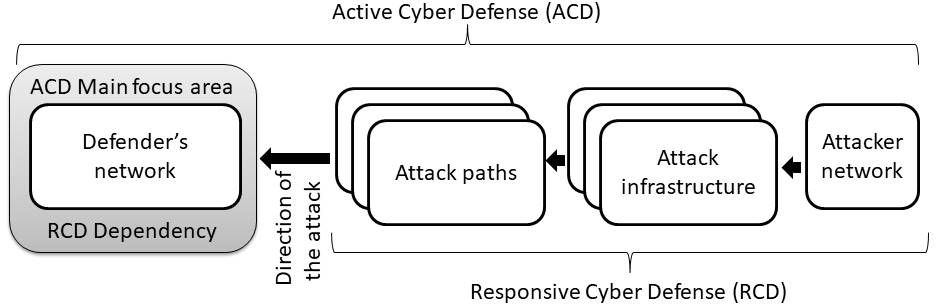
\includegraphics[width=0.8\textwidth]{./img/acd-rcd.jpg}
    \caption{Active and responsive cyber defence areas of engagement}
    \label{fig:acdrcd}
\end{figure}

% RCD requirements
Based on the related work, as presented in the chapter \ref{sec:rcd-work} and discussed here, the \gls{rcd} has at least the following requirements and characteristics:
\begin{enumerate}
    \item \textbf{Available.} The capability has to be permanently maintained and ready for deployment at the shortest notice possible.
    \item \textbf{Coordinated.} Has to be in response to an verified aggression and coordinated between the responders at various directions, such as, political, kinetic, or \gls{cnd}.
    \item \textbf{Integrated.} Compliant with the initial threat detection, assessment, and related \gls{acd} activities.
    \item \textbf{Synchronized.} Real-time as the attack has been detected and is still ongoing. Additionally, it can be asynchronous in cases when the attack has seized, but the artefacts have been identified through activities, such as, vulnerability assessment, threat hunting, digital forensics, or signature update on the threat detection and analysis systems.
    \item \textbf{Automated.} Maximum automation to allow the highest level of synchronization and minimize the time required for the early stages of response.
    \item \textbf{Asymmetric.} Every \gls{crt} action has to deliver the maximum possible effect. Which correlates with the high readiness and preparedness level of the \gls{crt}.
    \item \textbf{Omnipresent.} Ability to track and pursue adversary throughout the cyberspace with the highest flexibility possible.
    \item \textbf{Effective.} Capable of delivering the required impact, such as, destroy or reduce effectiveness of the attack, engage adversary by denial \& deception or a hack-back.
    \item \textbf{Independent.} \gls{crt} has to contain all the necessary capabilities to conduct the \gls{rcd}.
\end{enumerate}
This is not an exhaustive list and more characteristics could be applicable depending on the particular \gls{rcd} specifics and delivered effect requirements.